% !TEX root = ../../../main.tex
% 来源：中学数学实验教材·第三册（高中数学）
% 章节：不等式和解不等式 / 解不等式
% 原始文件：3.tex，行 1824-1851
% 类型：tikz
% ---
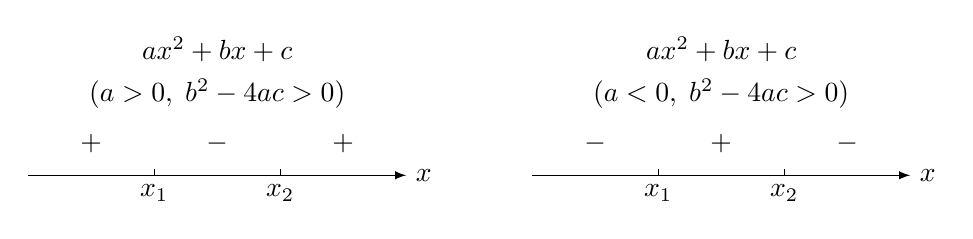
\begin{tikzpicture}[>=latex, scale=.8]
\begin{scope}
\draw[->] (0,0)--(6,0)node[right]{$x$};
\foreach \x/\xtext in {2/x_1,4/x_2}
{
    \draw (\x,0)node[below]{$\xtext$}--(\x,.1);
}
\foreach \x/\xtext in {1/+,3/-,5/+}
{
    \node at (\x,.5){$\xtext$};
}
\node at (3,2){$ax^2+bx+c$};
\node at (3,1.3){$(a>0,\; b^2-4ac>0)$};
\end{scope}
\begin{scope}[xshift=8cm]
\draw[->] (0,0)--(6,0)node[right]{$x$};
\foreach \x/\xtext in {2/x_1,4/x_2}
{
    \draw (\x,0)node[below]{$\xtext$}--(\x,.1);
}
\foreach \x/\xtext in {1/-,3/+,5/-}
{
    \node at (\x,.5){$\xtext$};
}
\node at (3,2){$ax^2+bx+c$};
\node at (3,1.3){$(a<0,\; b^2-4ac>0)$};
\end{scope}
\end{tikzpicture} 
